\documentclass{article}
\usepackage{neurips_2026}
\usepackage[utf8]{inputenc}
\usepackage[T1]{fontenc}
\usepackage{hyperref}
\usepackage{url}
\usepackage{booktabs}
\usepackage{amsmath,amssymb,amsthm}
\usepackage{graphicx}
\usepackage{xcolor}
\usepackage{microtype}
\newtheorem{proposition}{Proposition}
\newcommand{\E}{\mathbb E}
\newcommand{\Var}{\operatorname{Var}}
\newcommand{\IIDUniform}{4.48}
\newcommand{\IIDUniformRho}{0.848}
\newcommand{\IIDStrat}{3.98}
\newcommand{\IIDStratRho}{0.865}
\newcommand{\IIDSCFD}{3.77}
\newcommand{\IIDSCFDRho}{0.874}
\newcommand{\IIDRidge}{3.09}
\newcommand{\IIDRidgeRho}{0.902}
\newcommand{\IIDAIPW}{3.60}
\newcommand{\IIDAIPWRho}{0.866}
\newcommand{\IIDDifference}{3.89}
\newcommand{\IIDDifferenceRho}{0.848}
\newcommand{\FrontierUniform}{4.40}
\newcommand{\FrontierUniformRho}{0.664}
\newcommand{\FrontierStrat}{3.93}
\newcommand{\FrontierStratRho}{0.694}
\newcommand{\FrontierSCFD}{3.80}
\newcommand{\FrontierSCFDRho}{0.676}
\newcommand{\FrontierRidge}{7.51}
\newcommand{\FrontierRidgeRho}{0.499}
\newcommand{\FrontierAIPW}{3.82}
\newcommand{\FrontierAIPWRho}{0.656}
\newcommand{\FrontierDifference}{3.91}
\newcommand{\FrontierDifferenceRho}{0.664}
\newcommand{\GapUniform}{4.40}
\newcommand{\GapUniformRho}{0.664}
\newcommand{\GapStrat}{4.11}
\newcommand{\GapStratRho}{0.687}
\newcommand{\GapSCFD}{4.03}
\newcommand{\GapSCFDRho}{0.677}
\newcommand{\GapRidge}{12.30}
\newcommand{\GapRidgeRho}{0.380}
\newcommand{\GapAIPW}{4.14}
\newcommand{\GapAIPWRho}{0.651}
\newcommand{\GapDifference}{4.08}
\newcommand{\GapDifferenceRho}{0.664}
\newcommand{\CoreCellMinutes}{9.1}
\newcommand{\IRTFits}{260}
\newcommand{\IRTNonconverged}{0}
\newcommand{\IIDMIRT}{3.85}
\newcommand{\IIDMIRTMix}{3.27}
\newcommand{\FrontierMIRT}{9.43}
\newcommand{\FrontierMIRTMix}{6.93}

\title{Honest Residual Audits for Predicting LLM Benchmark Scores\\from Few Binary Responses}
\author{Anonymous Authors}
\begin{document}
\maketitle
\begin{abstract}
Historical item-level responses can reduce the cost of evaluating a new language model, but a good score predictor need not remain reliable beyond its source models. We study a simple design-based alternative: source-difficulty stratification followed by cross-fitted difference estimation (SCFD). Each queried half fits a target-specific response regression; the other half audits its residuals, with the correct finite-population weights. The resulting estimate is unbiased under the stated random sampling design, without requiring a correct response model. On thirteen public binary response matrices, with duplicate-group-disjoint splits and five seeds, fifty-item SCFD achieves macro mean absolute errors of \IIDSCFD{} and \FrontierSCFD{} percentage points under random and capability-frontier holdouts, compared with \IIDUniform{} and \FrontierUniform{} for uniform sampling. These are not universal gains: learned score regression is better under random holdout, simple stratification explains much of the improvement, and the honest estimator does not consistently improve rankings. Repeated-mask diagnostics and matched ablations expose the cost of residual honesty rather than establishing a new state of the art. All results, including unsuccessful optimization attempts, are reproducible on CPU.
\end{abstract}

\section{Introduction}
Repeatedly scoring model checkpoints, prompts, and inference settings on every item of a benchmark can dominate evaluation cost. A historical matrix of model-by-item correctness provides a tempting shortcut: ask a new model a small number of questions and infer its full score. Item selection and score reconstruction are distinct decisions. A representative subset may estimate an average directly; a response model may instead fill in the unobserved items or decode a full score from the observed signature.

These approaches exploit different assumptions. A score decoder learns relationships across historical model rows, whereas a target-specific item regression learns relationships across queried items. The former can interpolate well yet underestimate models beyond the source score range. An observed-sample residual correction does not automatically repair that problem if its predictor was fitted on the very residuals being averaged. In particular, an unpenalized regression intercept forces training residuals to sum to zero. The empirical questions are therefore not just which method has lower error, but which information is responsible for the gain, and what a claim of unbiasedness actually guarantees.

This paper applies a standard difference-estimation identity to this setting. Source responses define difficulty strata and fixed item covariates. Within each stratum, the query budget is split between a pilot and an audit. A pilot-trained response regression predicts the unobserved bank; a disjoint random audit corrects its residual total. Swapping the two roles uses all queried responses without evaluating residuals on their own training set. We call the resulting procedure \emph{stratified cross-fitted difference estimation} (SCFD). Its justification is finite-population randomization, not exchangeability between source and target model families.

The contribution is deliberately narrow: (i) an explicit honest estimator and information-boundary audit; (ii) a distinction between paper-level difference-estimator algebra and a pinned public implementation; and (iii) a controlled study of acquisition, reconstruction, bias, and ranking on thirteen real matrices. We do not claim to invent difference estimation, to exhaust the literature, or to improve all sparse-evaluation methods. Indeed, score ridge performs better in the interpolation setting, and honest auditing can lose to biased imputation. The target throughout is the \emph{flat mean of the supplied binary matrix}, not necessarily a benchmark's official scenario-weighted leaderboard score.

\section{Related work and positioning}
\paragraph{Representative questions and response models.}
\citet{vivek2023anchorpoints} select correlated anchor points using model confidence responses, and also identify nearest-source prediction as an important control. Binary correctness alone does not reproduce that confidence-based procedure. \citet{polo2024tinybenchmarks} provide binary correctness clustering, multidimensional item response theory (IRT), and generalized combinations of anchor and imputation estimates. \citet{kipnis2025metabench} combine IRT, information filtering, and generalized additive score reconstruction. These systems motivate separating the selector, predictor, and aggregate estimator. Our binary clustering and point-estimate IRT controls are labeled adaptations rather than exact reproductions of those full pipelines.

\paragraph{Learned assessment and acquisition.}
\citet{pacchiardi2024hundredinstances} predict success from a model's reference-response signature and item features, including genuinely unseen items. \citet{li2024activeevaluation} couple neural-process prediction with learned adaptive acquisition. Our matrix-only setting has historically observed item columns, no item-text embeddings, and nonadaptive queries. It cannot support a new-item prediction claim, nor does an inexpensive entropy or IRT heuristic stand in for their learned acquisition policy. \citet{balkir2026confidentrankings} address adaptive rankings with continuous scores and selective ties; ordinary Spearman correlation in our binary fixed-budget study is not their confidence guarantee.

\paragraph{Interpolation, extrapolation, and corrections.}
\citet{zhang2025missesthemark} compare benchmark predictors, including random-sampling score regression and a target-specific AIPW-style regression, and emphasize capability extrapolation. We use their explicitly permitted fixed data/code snapshot, not their reported numbers as our results. Our split groups exact duplicate rows, retains zero-score models, and uses different source fractions and query seeds. The proposed audit is a finite-sample sampling-theoretic adaptation. The principal empirical distinction is that a smaller signed bias can coexist with worse MAE, RMSE, or ranking. Restricted primary-source reading was used to respect an independent-research constraint; consequently no exhaustive priority claim is made.

\section{Setting and honest residual estimation}\label{sec:method}
Let $X\in\{0,1\}^{M\times N}$ contain fully observed source responses and let $y\in\{0,1\}^N$ be one fixed target row. Only queried entries of $y$ are available to an estimator. The estimand is
\begin{equation}\label{eq:target}
\mu=N^{-1}\sum_{i=1}^N y_i.
\end{equation}
All items retain their original multiplicities. We treat the historical response vector $x_i=X_{:,i}$ as an item covariate; no hidden target response is a feature.

\subsection{Why a same-sample correction is not an audit}
For a uniform query set $S$ of size $b$, write $U=S^c$ and let $q_i$ be predicted target correctness. A difference estimator has the algebraic form
\begin{equation}\label{eq:diff}
D=\bar q_{[N]}+\overline{(y-q)}_S
 =\bar y_S+\frac{N-b}{N}(\bar q_U-\bar q_S).
\end{equation}
When $q$ is fixed independently of the uniform draw, $D$ is design-unbiased. Fitting $q$ on $S$ does not meet that condition. Our target-specific nuisance regression, matching the pinned implementation's objective, is
\begin{equation}\label{eq:ridge}
(\hat c,\hat w)=\arg\min_{c,w}\sum_{i\in S}(y_i-c-x_i^\top w)^2+10\|w\|_2^2.
\end{equation}
The intercept is unpenalized; covariates are centered using the fitting items only. Thus $\overline{(y-q)}_S=0$ up to numerical precision. With this fit, Eq.~\eqref{eq:diff} becomes population-weighted imputation, not an independent residual check.

A separate implementation issue matters. The pinned public AIPW code computes
\begin{equation}\label{eq:pinned}
D_{\mathrm{pin}}=\bar q_U+\frac{N-b}{N}\overline{(y-q)}_S,
\end{equation}
which differs from Eq.~\eqref{eq:diff}. With an intercept it reduces to the mean prediction on $U$, omitting the observed-population contribution. We retain both \emph{AIPW--pinned} and \emph{AIPW--population}, the latter using Eq.~\eqref{eq:diff}. This discrepancy is not attributed to a new statistical principle. Unit tests compare our vectorized implementation with the actual pinned classes.

\subsection{Source-defined selection and disjoint audits}
Sort items by their source mean $d_i=M^{-1}\sum_m X_{mi}$, breaking ties by item index, and divide the ordered list into $H=5$ nearly equal-sized strata $U_h$. Let $N_h=|U_h|$. Allocate $\lfloor b/H\rfloor$ queries to each stratum and distribute any remainder by a seeded label-independent permutation. Within each stratum, draw ordered items uniformly without replacement. The first $p_h=\lfloor b_h/2\rfloor$ form $P_h$ and the remaining $a_h=b_h-p_h$ form $A_h$. Every studied budget has $p_h,a_h\geq1$.

Fit Eq.~\eqref{eq:ridge} using $P=\cup_hP_h$ alone, giving $q^P$. Define the directional estimator
\begin{equation}\label{eq:honest}
T(P\!\to\!A)=\frac1N\left[\sum_{i\in P}y_i+\sum_{i\notin P}q_i^P
+\sum_h(N_h-p_h)\overline{(y-q^P)}_{A_h}\right].
\end{equation}
The correction uses the complement of the \emph{pilot}, including the audit, not just the unqueried items. Independently fitting the swapped role gives $T(A\!\to\!P)$; SCFD is their fixed half-average. This remains valid for unequal fold sizes, although at odd budgets it need not reduce to the raw sample mean for a constant nuisance. The query cost is $|P\cup A|=b$, not two evaluations per item. Uniform CFD is the same estimator with a single stratum.

\begin{proposition}[Design unbiasedness]\label{prop:unbiased}
Fix the source matrix, strata, and target row. Draw the disjoint sets with the fixed, feasible sizes above. Let each fitted prediction vector be a finite deterministic function of sources, its own pilot membership and labels only, or a randomized function independent of audit membership with integrable predictions. Then $\E[T(P\to A)]=\mu$, and the fixed half-average SCFD is unbiased. This statement concerns ideal random sampling, not a guarantee that a finite list of pseudorandom seeds has zero empirical bias.
\end{proposition}
\paragraph{Proof sketch.}
Conditional on the pilot and any independent learner randomness, $q^P$ is fixed and $A_h$ is uniform over $U_h\setminus P_h$. Its residual mean therefore estimates that complement's residual mean. Multiplying by $N_h-p_h$ cancels the predicted complement total in Eq.~\eqref{eq:honest}. The remaining total is exactly $\sum_i y_i$. Apply the same argument to the swapped direction and use linearity. Appendix~\ref{app:proof} gives the full proof, variance, and boundary cases.

The estimator is not necessarily unbiased conditional on the realized union $S$, does not require source/target distributional agreement, and is not clipped to $[0,1]$. Source-only preprocessing of full item covariates is legal; any dependence of $q^P$ on audit membership, even without audit labels, is not covered. The two directions share queried responses and are dependent. Their individual variance formulas cannot be averaged as independent error estimates, and no calibrated score or rank interval is claimed here.

\section{Experimental protocol}\label{sec:protocol}
\paragraph{Data and split integrity.}
We use all thirteen specified LLM matrices in repository commit \texttt{55faff496947789f94e6b5908c77cbc3e84f81ad}: seven Open LLM Leaderboard banks and six HELM-derived banks (Appendix~\ref{app:data}). They have 79--448 model rows and 437--12,032 item columns. Every entry is finite and binary. Exact duplicate response rows are grouped before splitting, preventing an identical full response signature from appearing in both source and target sets. Grouping is an oracle split-only operation, not a deployable feature or evidence of family independence. All rows, constant items, and duplicate columns remain. In particular, all 53 all-zero OpenLLM-MATH rows remain rather than censoring observed failures.

For \emph{random group holdout} (IID shorthand), randomly assign 70\% of unique groups to sources, rounded down. For \emph{frontier holdout}, order groups by their flat full score and choose the score-tie-block boundary nearest 70\%; the higher-scoring groups are targets. Full scores enter only this retrospective split construction and final evaluation, never acquisition or prediction. A stronger \emph{gap} sensitivity uses the bottom 50\% as sources and top 30\% as targets, leaving an unused middle region. These are oracle capability stress tests, not temporal or family-held-out evaluation.

\paragraph{Budgets, seeds, and controls.}
The primary budget is $b=50$; secondary budgets are $10,25,100$. Seeds 0--4 control reproducible source and query streams. Frontier membership is unchanged across seeds: these are five query designs, not five independent frontier populations. Query masks are shared across target models and across methods within the uniform or stratified track. Uniform masks are nested across budgets; stratified masks need not be. Anchor methods form a separate acquisition track. Both tracks use the same number of queried labels. A $2b$ uniform reference is explicitly higher-cost.

Controls include uniform and source-stratified means; fixed source-item difference estimators; score ridge fitted across source \emph{model rows} with RidgeCV penalties $\{0.1,1,10\}$; the two target-item AIPW variants; regularized Rasch 1PL; binary correctness MiniBatchKMeans anchors with actual-item representatives and cluster weights; and anchors with the same Rasch decoder. SCFD ablations remove stratification, symmetrization, audit correction, or residual honesty while retaining the pilot fits. Penalties and five strata are fixed, not target-tuned. The stronger multidimensional comparator in Appendix~\ref{app:mirt} was added after the primary analysis, with source-only fitting and calibration. No proposed setting or primary contrast was revised. After self-review, an inexpensive nearest-source control was also added on the saved uniform queries (Appendix~\ref{app:settings}).

\paragraph{Metrics and uncertainty.}
Within a bank, primary metrics weight each target duplicate group equally; original-row weighting is a sensitivity. We macro-average bank MAEs and signed errors, and define macro RMSE as the square root of the mean bank MSE. Spearman $\rho$, Kendall $\tau_b$, and pair agreement are computed within each bank, never across unrelated tasks; true ties are excluded from pair agreement and prediction ties receive half credit. For ordering metrics only, truth and predictions are rounded to ten fractional decimal places to restore numerical ties; raw scores are retained for error metrics. This policy repaired a self-review finding in which machine-precision residual sums broke common-offset rank invariance (Appendix~\ref{app:uncertainty}). Correlations are averaged over banks and seeds.

We report five-seed variability and percentile 95\% bootstrap intervals from 10,000 resamples of the thirteen \emph{seed-averaged bank means}. Shared model pools, related tasks, shared masks, and repeated targets make these \emph{descriptive bank-resampling intervals}, not population-valid independent-benchmark inference or per-model score intervals. Four prespecified SCFD contrasts (two regimes, uniform and stratified means) have paired bank sign-flip tests with Holm correction; their independence/symmetry assumptions are doubtful here, so they are sensitivity summaries, not claims of confirmatory significance (Appendix~\ref{app:uncertainty}). To examine bias separately, a fixed-source diagnostic uses 200 new query masks at budgets 10 and 100 on the largest and median-sized banks, MMLU-Pro and GSM, and six target groups selected independently of method error. Monte Carlo standard errors are computed over masks, preserving shared-target error dependence.

\section{Results}\label{sec:results}
\begin{table}[t]
\caption{Budget-50 group-weighted performance. Errors are percentage points; lower is better, higher $\rho$ is better. Brackets are descriptive 95\% bank-bootstrap intervals after averaging five seeds. Approximate binary anchors and Rasch are adaptations, not full published systems.}\label{tab:main}
\centering\scriptsize\setlength{\tabcolsep}{3pt}\begin{tabular}{lrrrrrr}
\toprule
Method & IID MAE [CI] & Frontier MAE [CI] & IID RMSE & Front. RMSE & $\rho$ IID & $\rho$ Front. \\
\midrule
Uniform & 4.48 [3.99, 4.86] & 4.40 [3.92, 4.86] & 5.75 & 5.60 & 0.848 & 0.664 \\
Stratified mean & 3.98 [3.51, 4.39] & 3.93 [3.50, 4.40] & 5.12 & 5.00 & 0.865 & 0.694 \\
Item difference & 3.89 [3.44, 4.28] & 3.91 [3.52, 4.29] & 5.01 & 4.99 & 0.848 & 0.664 \\
Stratified difference & 3.91 [3.45, 4.32] & 3.83 [3.37, 4.32] & 5.05 & 4.89 & 0.865 & 0.694 \\
Score ridge & 3.09 [2.63, 3.54] & 7.51 [6.16, 8.95] & 4.06 & 9.08 & 0.902 & 0.499 \\
Stratified score ridge & 3.02 [2.57, 3.45] & 7.37 [6.05, 8.77] & 4.04 & 8.89 & 0.914 & 0.532 \\
AIPW--pinned & 3.61 [3.21, 3.97] & 3.86 [3.51, 4.22] & 4.64 & 4.89 & 0.865 & 0.655 \\
AIPW--population & 3.60 [3.21, 3.95] & 3.82 [3.46, 4.18] & 4.63 & 4.84 & 0.866 & 0.656 \\
Rasch 1PL & 3.74 [3.30, 4.15] & 3.76 [3.41, 4.10] & 4.85 & 4.80 & 0.848 & 0.664 \\
Binary anchors & 4.47 [3.77, 5.41] & 9.15 [5.43, 13.35] & 6.06 & 14.93 & 0.872 & 0.608 \\
Uniform CFD & 3.81 [3.41, 4.16] & 3.90 [3.52, 4.29] & 4.88 & 4.96 & 0.855 & 0.648 \\
SCFD & 3.77 [3.35, 4.10] & 3.80 [3.36, 4.26] & 4.84 & 4.86 & 0.874 & 0.676 \\
MIRT--5 (added) & 3.85 [3.18, 4.50] & 9.43 [7.91, 11.24] & 5.00 & 10.69 & 0.899 & 0.546 \\
MIRT mixture (added) & 3.27 [2.83, 3.68] & 6.93 [5.67, 8.44] & 4.26 & 8.23 & 0.897 & 0.624 \\
Nearest source (added) & 4.16 [3.23, 5.17] & 9.26 [7.23, 11.56] & 6.04 & 11.41 & 0.854 & 0.290 \\
\bottomrule
\end{tabular}

\end{table}

\paragraph{The best reconstruction depends on the split.}
Table~\ref{tab:main} shows that score ridge achieves \IIDRidge{} pp random-holdout MAE but degrades to \FrontierRidge{} pp on frontier targets. It learns a source-population score mapping, whereas target-item regressions can change with each target's observed responses. SCFD improves uniform sampling from \IIDUniform{} to \IIDSCFD{} pp in random holdout and from \FrontierUniform{} to \FrontierSCFD{} pp on the frontier. Yet it is not the best overall estimator: score ridge is better in random holdout, and Rasch and AIPW--population are close frontier competitors. The coefficient repair changes pinned AIPW only modestly in these data; the implementation discrepancy is real, but it is not the dominant empirical effect. The added source-calibrated multidimensional IRT mixture has MAE \IIDMIRTMix{} pp in random holdout and \FrontierMIRTMix{} pp on the frontier; its extra expressivity does not remove this stress-test failure.

\begin{figure}[t]
\centering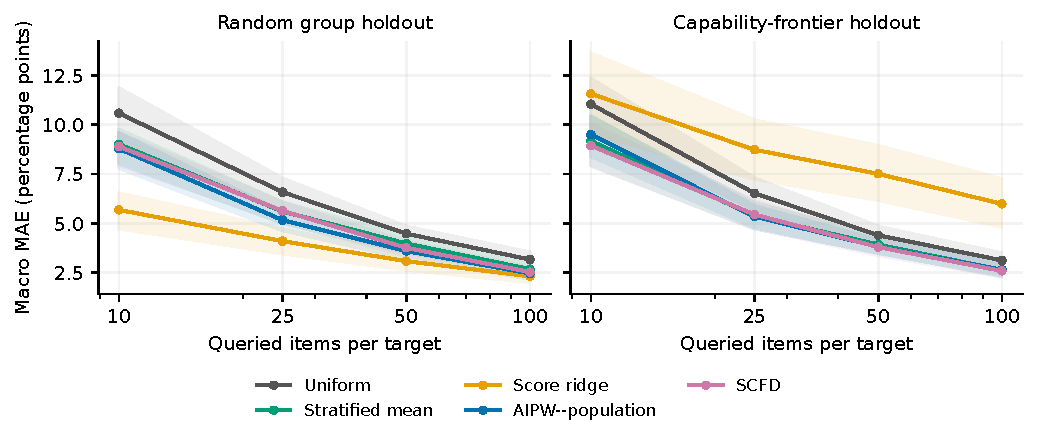
\includegraphics[width=\linewidth]{figures/budget_curves.pdf}
\caption{MAE versus query budget for five original methods (all configurations are tabulated in the appendix). Shading shows the same descriptive bank-resampling intervals as Table~\ref{tab:main}; it does not represent uncertainty in an individual predicted score. Source score regression improves interpolation but remains less accurate on frontier targets over the studied budgets.}\label{fig:budgets}
\end{figure}

\paragraph{Simple selection accounts for much of the improvement.}
Figure~\ref{fig:budgets} shows the finite-budget trends. Stratified means achieve \IIDStrat{} and \FrontierStrat{} pp MAE. Relative to them, SCFD's absolute reductions are substantially smaller than its reductions over uniform. The paired frontier SCFD-minus-uniform difference is $-0.60$ pp with descriptive interval $[-1.00,-0.19]$; against stratified means it is $-0.13$ pp with interval $[-0.23,-0.02]$. The latter contrast has Holm-adjusted sign-flip $p=0.0515$, illustrating that favorable bootstrap endpoints should not be turned into a strong inferential claim. These summaries also ignore between-family deployment uncertainty. The complete seed deltas, assumptions, and four comparisons are in Appendix~\ref{app:uncertainty}. Fixed stratified difference is an even stronger simple honest control: its frontier MAE is 3.83 pp versus 3.80 for SCFD, only a 0.03 pp increment from target-specific fitting; the corresponding random-holdout increment is 0.15 pp. This near-equivalence is a central negative result, not evidence that the learned pilot is practically necessary.

\begin{figure}[t]
\centering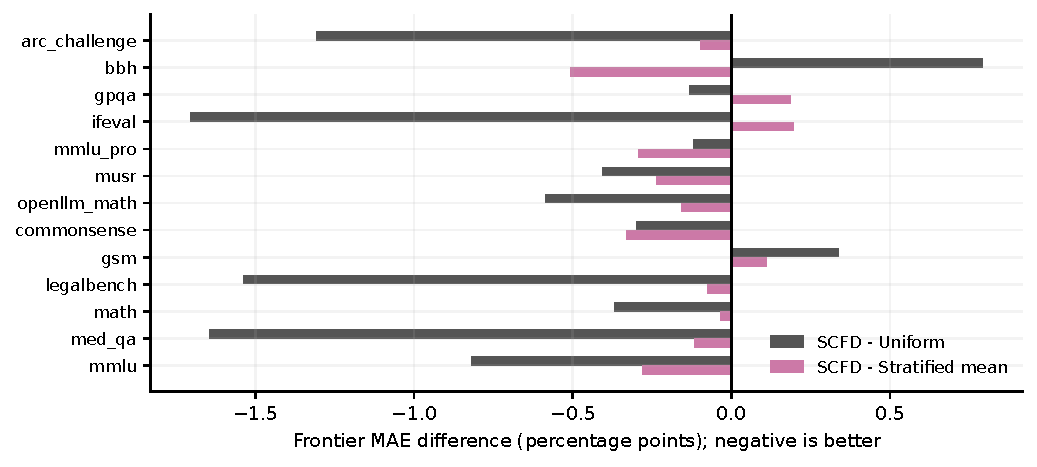
\includegraphics[width=\linewidth]{figures/paired_effects.pdf}
\caption{Budget-50 frontier effects after averaging five query seeds. Negative differences favor SCFD. Gains over uniform are heterogeneous, and several banks lose to simple stratification. There is no cross-task universal improvement.}\label{fig:effects}
\end{figure}

\paragraph{There are observable failures, not just a favorable macro-average.}
SCFD beats uniform in eleven of thirteen frontier banks but loses on BBH and GSM (Figure~\ref{fig:effects}, full values in Appendix~\ref{app:full}). Under frontier holdout, stratified mean has higher macro Spearman correlation (\FrontierStratRho{}) than SCFD (\FrontierSCFDRho{}), despite its slightly higher MAE. Aggregate score accuracy therefore does not imply better ordering. Larger uniform samples are also competitive: the $2b$ reference uses twice as many responses and must not be presented as a budget-matched win. The sharp frontier losses of binary weighted anchors show that source-space representativeness alone is not sufficient; decoding the same anchors with Rasch changes the result substantially (Appendix~\ref{app:full}).

\begin{table}[t]
\caption{Matched mechanism ablations at budget 50. All errors are pp; signed frontier error is not a bias estimate over all item designs. The no-audit variant uses both pilot fits and therefore the same total $b$ labels; each fit uses only its own half, and their population-imputation estimates are averaged without residual auditing. The contaminated diagnostic reuses pilot residuals and has no honesty guarantee.}\label{tab:ablation}
\centering\small\setlength{\tabcolsep}{4pt}\begin{tabular}{lrrrr}
\toprule
Method & IID MAE & Front. MAE & Front. bias & Front. RMSE \\
\midrule
Uniform & 4.48 & 4.40 & -0.05 & 5.60 \\
Stratified mean & 3.98 & 3.93 & -0.20 & 5.00 \\
Stratified difference & 3.91 & 3.83 & -0.20 & 4.89 \\
SCFD: no audit & 3.58 & 3.87 & -1.41 & 4.95 \\
SCFD: contaminated & 3.57 & 3.71 & -0.82 & 4.73 \\
SCFD: one direction & 5.19 & 5.50 & -0.52 & 7.05 \\
Uniform CFD & 3.81 & 3.90 & -0.18 & 4.96 \\
SCFD & 3.77 & 3.80 & -0.26 & 4.86 \\
\bottomrule
\end{tabular}

\end{table}

\paragraph{Honesty is not an MAE-optimality guarantee.}
Removing one audit direction markedly worsens error (Table~\ref{tab:ablation}); swapping the roles recovers much of that loss. However, contaminated residual correction and unaudited imputation are better than SCFD in some conditions. They share the same pilot nuisance fits, isolating the estimator's bias--variance trade-off rather than comparing unrelated models. Likewise uniform CFD versus stratified SCFD isolates the selection design. None of these comparisons supports a claim that every proposed component is indispensable for optimal prediction. Honest correction is valuable when protection against model misspecification is the objective, but its smaller pilot sets and residual noise carry a cost.

\begin{figure}[t]
\centering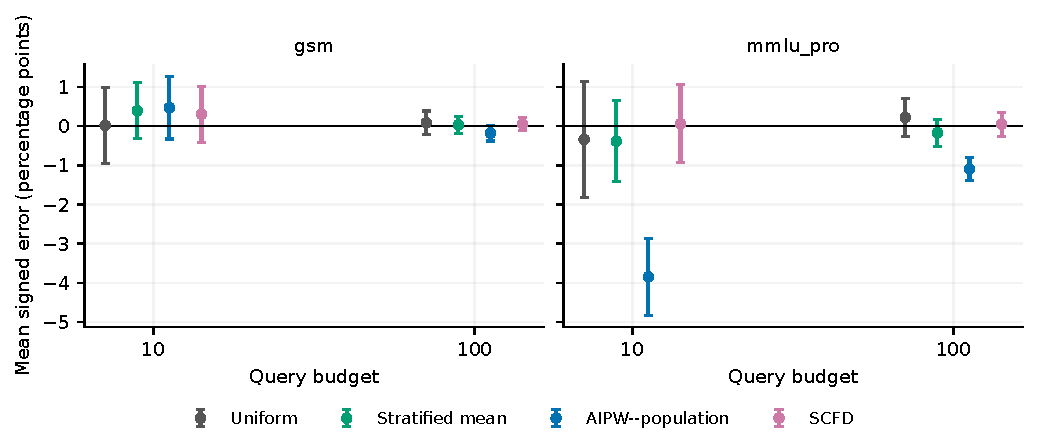
\includegraphics[width=\linewidth]{figures/bias_diagnostics.pdf}
\caption{Fixed-source frontier diagnostics: mean signed error across six fixed target groups and 200 fresh masks, with $\pm2$ Monte Carlo standard errors. Errors shared by targets under the same mask are retained when computing these bars. These are not confidence intervals for unseen model populations.}\label{fig:bias}
\end{figure}

\paragraph{Repeated masks distinguish a theorem from a five-seed average.}
The repeated-mask panel in Figure~\ref{fig:bias} conditions on fixed source and target rows. Honest estimators fluctuate around the full score; the full-query target regression can retain directional error. The plotted quantity averages signed errors, so opposite target biases can cancel. We therefore also release targetwise diagnostics, within-target variance, and the exact empirical MSE decomposition (Appendix~\ref{app:diagnostics}). The squared empirical bias includes finite-mask Monte Carlo noise; it is not an unbiased estimate of squared design bias. We do not infer exact unbiasedness from a small plotted error bar: the proposition supplies the guarantee, whereas the experiment measures its practical cost. No score-interval coverage study or adaptive stopping experiment was completed.

\paragraph{Sensitivity and compute.}
Original-row weighting and the stronger bottom-50/top-30 gap split are reported alongside the group-weighted results. The latter yields SCFD MAE \GapSCFD{} pp, uniform \GapUniform{} pp, and score ridge \GapRidge{} pp. Changing the source population alters learned estimators; it does not strengthen a randomization theorem into a model-generalization theorem. The original main grid contains 130 source-split/seed cells and 8,840 method-budget outputs, including ablation configurations and the explicitly extra-cost reference. It used \CoreCellMinutes{} summed cell-minutes on CPU; wall time, stronger IRT cost, optimizer repairs, and reproduction commands are in Appendix~\ref{app:repro}. No LLM was rerun and no paid API was called.

\section{Discussion, limitations, and broader impact}\label{sec:limitations}
The practical choice depends on the intended safeguard. If new models resemble the source population and point accuracy is paramount, a source-trained score decoder can be preferable. If capability shift is plausible, uniform or difficulty-stratified sampling supplies a transparent fallback; SCFD provides a valid mean estimator under its random item design without promising lower error on every bank. Increasing the query budget can be more useful than replacing a simple estimator with a complex one. Ranking-sensitive deployments require rank-specific checks: our frontier results explicitly contradict a monotone relationship between MAE and ranking quality.

Our study has important limits. Exact-response grouping is not family independence, contamination detection, or a chronological deployment simulation. The thirteen banks reuse model pools and are not independent samples from a benchmark universe. Five seeds provide coarse query variability, and the diagnostic banks and six targets do not establish population-wide calibration. Flat binary means may differ from official subject-weighted scores. The matrices contain repeated columns and endpoint rows whose upstream causes cannot be resolved from correctness alone; retaining them is a transparent choice, not a quality certification. The source-specific ridge penalty and pilot split may be suboptimal; no target-driven optimization was attempted. Anchor and IRT adaptations do not reproduce confidence-based anchors, Bayesian tinyBenchmarks, metabench, or neural RL acquisition. Accordingly this is a protocol and estimator study, not a comprehensive state-of-the-art comparison. Ideal design unbiasedness also presumes proper random sampling and audit isolation; deterministic finite PRNG seed lists are a reproducibility device, not an exact sampling distribution.

Sparse evaluation can save compute and broaden access to model assessment. It can also miss rare failures, enable public-subset overfitting, or present small score differences with unjustified precision. Reduced average-score error is not a safety, fairness, robustness, or construct-validity guarantee. Randomized refresh, full evaluations before consequential decisions, and explicit disclosure of uncertainty are appropriate safeguards. This artifact releases correctness-derived summaries and code, not model weights, private records, or new scraped content.

\section{Conclusion}
Source history helps, but acquisition, decoding, and estimator honesty should be evaluated separately. SCFD applies a finite-population residual audit to sparse binary LLM evaluation and improves uniform sampling in the studied macro-averages. Much of the gain is already available from simple stratification, learned interpolation can be more accurate, and the ranking result is not uniformly favorable. The main recommendation is a controlled, source-only comparison with a strong random-sampling fallback, not unconditional adoption of the proposed estimator.

\clearpage
\bibliographystyle{plainnat}
\bibliography{references}
\clearpage
\appendix
\section{Full design argument and boundary cases}\label{app:proof}
Fix $X$, $y$, the partition $U_1,\ldots,U_H$, and feasible positive integers $p_h,a_h$ with $p_h+a_h\leq N_h$. Within each stratum, choose a disjoint ordered pair of subsets $(P_h,A_h)$ uniformly among all pairs of those sizes, independently across strata. Random allocation of the leftover query counts is also allowed: condition on those label-independent counts first. Let $\mathcal G_P$ contain $P$, its observed labels, and any independent learner randomness. Require $q^P$ to be measurable with respect to this information and fixed source/item covariates, not audit membership. In particular, centering or hyperparameter selection using $P\cup A$ is not automatically permitted. Deterministic finite ridge predictions satisfy the integrability condition below.

Define $R_h=U_h\setminus P_h$, $M_h=N_h-p_h$, and $e_i=y_i-q_i^P$ on $R_h$. Conditional on $\mathcal G_P$, each $A_h$ is a uniform $a_h$-subset of $R_h$, and hence
\begin{equation}\label{eq:auditexpect}
\E\!\left[\overline e_{A_h}\mid\mathcal G_P\right]
=M_h^{-1}\sum_{i\in R_h}e_i.
\end{equation}
Substitute Eq.~\eqref{eq:auditexpect} into Eq.~\eqref{eq:honest}:
\begin{align}
\E[T(P\to A)\mid\mathcal G_P]
&=N^{-1}\left[\sum_{i\in P}y_i+\sum_{i\notin P}q_i^P+
\sum_h\sum_{i\in R_h}(y_i-q_i^P)\right]\\
&=N^{-1}\sum_i y_i=\mu.\label{eq:proof}
\end{align}
For a randomized learner, $\E\sum_i|q_i^P|<\infty$ is sufficient to take the outer expectation. An unrestricted unbounded randomized predictor need not be integrable, so the claim is not made for every conceivable randomized learner. Reversing the roles is legitimate because, conditional on $A$, the corresponding $P_h$ is uniform on its stratum complement. Each direction has marginal expectation $\mu$, and any fixed convex combination does too. Unequal fold sizes therefore do not invalidate the half-average; equal weighting was fixed before results rather than selected for target performance. The half-average is not generally unbiased conditional on $P$ or on the realized union $S$ because its second direction has a different conditioning argument.

For $M_h>1$ define
\begin{equation}\label{eq:residualvar}
S_{e,h}^2=(M_h-1)^{-1}\sum_{i\in R_h}(e_i-\bar e_{R_h})^2.
\end{equation}
The without-replacement sample-mean variance is $(1-a_h/M_h)S_{e,h}^2/a_h$. Conditional independence across stratum audit draws gives
\begin{equation}\label{eq:dirvar}
\Var(T(P\to A)\mid\mathcal G_P)
=N^{-2}\sum_h\frac{M_h^2}{a_h}\left(1-\frac{a_h}{M_h}\right)S_{e,h}^2.
\end{equation}
If $a_h=M_h$, the complement is a census and that contribution is exactly zero. When $M_h=1$, feasibility forces $a_h=1$; define its variance contribution as zero without evaluating an undefined denominator. Empty audit strata are forbidden. The two-direction variance contains a covariance term,
\begin{equation}
\Var\!\left(\frac{T_1+T_2}{2}\right)
=\frac14\{\Var(T_1)+\Var(T_2)+2\operatorname{Cov}(T_1,T_2)\},
\end{equation}
which cannot be discarded merely because the pilot sets are disjoint. No practical confidence interval for SCFD is derived or claimed.

\paragraph{What is and is not validated.}
The unit tests enumerate all feasible ordered pilot/audit allocations for tiny fixed binary populations, including unequal folds, all-zero/all-one rows, a full census, and a stratified example. These are synthetic \emph{code correctness tests}, not evidence substituted for a real benchmark experiment and not a proof of the general proposition. Other tests compare the exact pinned Ridge and AIPW classes numerically, verify the finite-population identity, check duplicate-group separation, verify hidden-label invariance, and check finite endpoint Rasch predictions. The initial nine tests passed; the final twelve-test suite adds numerical rank-invariance, nearest-source tie/retention, and invalid-budget regression checks. Validity of the theoretical sampling distribution presumes an actual randomized design: the reproducible experiment uses a finite set of pseudorandom streams, not an exhaustive uniform randomization distribution. Distinct seed namespaces are used for split construction, uniform queries, stratified queries, inner IRT calibration, and diagnostic masks; coupled run indices should not be interpreted as independent random populations.

\section{Data audit and preprocessing}\label{app:data}
\begin{table}[h]
\caption{Actual data dimensions and seed-0 frontier group counts. ``Unique'' means exact response groups, not independent model families. Constant items and zero-score rows remain.}\label{tab:data}
\centering\scriptsize\setlength{\tabcolsep}{4pt}\begin{tabular}{lrrrrrrr}
\toprule
Bank & Rows & Items & Unique & Zero rows & Const. items & Src. groups & Tgt. groups \\
\midrule
arc\_challenge & 218 & 1172 & 209 & 0 & 32 & 146 & 63 \\
bbh & 446 & 5761 & 425 & 0 & 0 & 297 & 128 \\
gpqa & 447 & 1192 & 424 & 0 & 0 & 298 & 126 \\
ifeval & 448 & 541 & 427 & 0 & 7 & 299 & 128 \\
mmlu\_pro & 448 & 12032 & 425 & 0 & 1 & 297 & 128 \\
musr & 448 & 756 & 427 & 0 & 10 & 297 & 130 \\
openllm\_math & 447 & 894 & 375 & 53 & 119 & 263 & 112 \\
commonsense & 83 & 500 & 82 & 0 & 0 & 57 & 25 \\
gsm & 83 & 1000 & 83 & 0 & 3 & 58 & 25 \\
legalbench & 79 & 2047 & 79 & 0 & 53 & 55 & 24 \\
math & 83 & 437 & 83 & 0 & 1 & 59 & 24 \\
med\_qa & 83 & 1000 & 82 & 0 & 2 & 57 & 25 \\
mmlu & 83 & 567 & 82 & 0 & 1 & 57 & 25 \\
\bottomrule
\end{tabular}

\end{table}
The input files are the thirteen named binary matrices in \texttt{data/scores/} at the fixed commit. SHA-256 hashes, duplicate-row/column counts, score ranges, and matrix means are in \texttt{artifacts/data\_audit.csv}. We do not execute upstream downloads of gated per-model detail datasets. Joblib files are loaded only from the permitted trusted fixed repository; untrusted joblib/pickle files should never be loaded. The source archive's MIT license covers the packaged assets under the provided data brief; upstream task and evaluation artifacts can have different terms. We distribute the artifact's new code separately, preserve the vendor copyright notice, and supply pinned download instructions rather than asserting a new license over all upstream benchmark content.

Source rows retain their multiplicities during training; primary evaluation gives each target response group equal weight. Thus grouping controls direct duplication leakage but is not source reweighting or an ancestry inference. Full target response vectors and group fingerprints are accessible only to the split builder and evaluator. Estimator functions receive the source matrix, queried item indices, and the corresponding target labels. The runner saves exact source/target row memberships and query indices. Scores used for frontier ordering are not passed to predictors. The lower50/upper30 gap sensitivity chooses boundaries at complete score-tie blocks nearest those fractions. Realized counts can differ slightly from nominal fractions. IID source assignments change with seed; frontier membership does not. No metadata-supported family, date, or future-release claim is made.

\section{Detailed estimators and hyperparameters}\label{app:settings}
\paragraph{Sample and fixed-difficulty controls.}
Uniform sampling uses one label-independent item permutation and nested prefixes. The fixed source-item control is $\bar d_{[N]}+\overline{(y-d)}_S$. For stratified queries it uses $\bar d_{[N]}+\sum_h(N_h/N)\overline{(y-d)}_{S_h}$. The stratified sample mean is $\sum_h(N_h/N)\bar y_{S_h}$, not the unweighted pooled mean when bank or quota sizes differ. Each is design-unbiased for its specified sampling design. With shared uniform queries, adding a fixed item-difficulty offset to every target cannot change that run's ordering; it can nevertheless change score errors.

\paragraph{The two ridge orientations.}
Score ridge takes source model rows as observations, source full means as labels, and queried responses as features. RidgeCV uses its default leave-one-out criterion and penalties $0.1,1,10$, with an unpenalized intercept and no normalization. Target-item regression instead uses sampled items as observations and source model response vectors as features, fitted anew for each target with summed squared loss and penalty 10. Pilot fitting uses the same penalty as the full-query control; reducing the number of pilot items changes the effective regularization per observation, which is part of the trade-off, not a tuned advantage. The implementation uses a centered dual solve of size at most $b\times b$ and batches target right-hand sides. Full-bank prediction sums are obtained from source covariate sums; no hidden target entries enter them.

\paragraph{Rasch adaptation.}
The source model is $p_{mi}=\sigma(\theta_m-\beta_i)$ with objective summed Bernoulli negative log-likelihood plus $\sum_m\theta_m^2/8+\sum_i\beta_i^2/18$. We use damped, step-limited Newton updates (damping $0.5$, individual step bound 1). The common-shift likelihood invariance is resolved by exactly minimizing the quadratic prior along $(\theta,\beta)\mapsto(\theta+c,\beta+c)$. The fixed cap is 200 iterations and the maximum update tolerance is $10^{-6}$; final main/gap fits all met tolerance, with at most 62 iterations. For a target, optimize its single ability from queried responses with prior $\theta^2/8$, step bound 1 and cap 80, then average actual queried outcomes and imputed unqueried probabilities. This is not multidimensional Bayesian IRT.

\paragraph{Binary anchors.}
MiniBatchKMeans operates on $N$ source-correctness vectors in $\mathbb R^M$, with Euclidean distance, $b$ clusters, three initializations, batch size 1,024, cap 100, and reassignment ratio zero. Choose the nearest as-yet-unused actual item to each centroid; deterministic item order resolves ties. Reassign all bank items to their nearest selected representative and weight by cluster size. Empty representative clusters get zero weight but the query union still has exactly $b$ distinct items. Unlike the original confidence-correlation medoids, this is a linear-storage correctness adaptation. We separately apply the identical source-calibrated Rasch decoder to those anchors to isolate part of the reconstruction effect. Deterministic anchors are not covered by the audit theorem.

\paragraph{Nearest-source control added after review.}
The self-review identified its omission from the initial comparison. For each target, find the minimum Hamming distance to source response signatures on the uniform query set. Average the unqueried response totals of all exactly tied nearest source rows, retain the actual queried target outcomes, and divide the combined total by $N$. This fixed tie-averaged binary adaptation uses no tuning and no full target score. It was run for all original 130 main cells and four budgets on their saved masks; gap experiments were not extended. The addition does not alter any frozen contrast. The comparison still does not exhaust all plausible decoders.

\paragraph{Matched ablations.}
The one-direction SCFD estimate uses $T(P\to A)$ only. The unaudited diagnostic is the half-average of $[\sum_P y+\sum_{i\notin P}q_i^P]/N$ and its swapped analogue. It does not consume its audit half's labels when constructing each directional prediction; the symmetrized estimate nevertheless uses both halves and has total label cost $b$. The contaminated-residual diagnostic uses each pilot fit but corrects with the pooled stratified residual mean on $P\cup A$, thus deliberately mixing training and held-out residuals. Its lower error in some cells is reported rather than suppressed; it is not claimed unbiased. All final scores are unbounded estimates and are not clipped. Out-of-range rates and errors at the original model-row weighting are included in the CSVs.

\section{Stronger multidimensional comparator added after primary analysis}\label{app:mirt}
A missing strong IRT control was identified after the frozen primary analysis. We therefore ran a separate complete uniform-query comparator grid; \texttt{logs/irt\_comparator\_amendment.md} records this timing. No proposed-method setting or prespecified contrast changed. The source model is
\begin{equation}
p_{mi}=\sigma(\theta_m^\top\alpha_i-\beta_i),\qquad \theta_m,\alpha_i\in\mathbb R^5.
\end{equation}
The rank is fixed at five before its target scoring, not chosen from target error. Optimize summed Bernoulli negative log-likelihood plus $\|\Theta\|_F^2/2+\|A\|_F^2/2+\|\beta\|_2^2/18$ with L-BFGS-B, relative objective tolerance $10^{-9}$, gradient tolerance $10^{-4}$, history 10, and cap 1,000. Initialization uses the top-five eigenvectors of the source-centered row covariance; item loadings are source projections and difficulty starts at the smoothed marginal logit. The bilinear fit is nonconvex; optimizer success is a numerical stopping status, not a global-optimum certificate. Targets have an independent standard-normal ability prior and are fitted only on queried outcomes, followed by observed-plus-imputed population aggregation. Target Newton updates start at zero, have a 60-iteration cap, step-norm bound 2, and maximum raw-step tolerance $10^{-7}$. A separate target convergence certificate was not saved; the 260 reported success statuses refer only to source and inner-source fits.

For a source-calibrated mixture, reserve 20\% of source response groups with a seeded random inner split, fit the IRT model only on the other 80\%, and infer the inner validation groups from the same uniform query contexts. Let $B$ be the mean absolute validation score error, and $V$ the mean Bernoulli row variance in inner sources. Use $\lambda=B^2/(V/b+B^2)$ and report $\lambda\bar y_S+(1-\lambda)\hat\mu_{\mathrm{MIRT}}$. Refit item parameters on all outer sources for final target inference. This adapts the generalized-IRT bias--variance idea to these actual query budgets; it is not the original hierarchical variational tinyBenchmarks training or an exact replication of its half-item calibration heuristic. Inner validation rows are absent from item fitting and preprocessing. The strong comparator adds two estimates per main cell; its full results appear in Table~\ref{tab:main} and Tables~\ref{tab:all-iid}--\ref{tab:all-frontier}.

Initial four smoke cells used cap 250 and several fits hit that cap. Only source optimization statuses were inspected before increasing it to 1,000 and rerunning the entire comparator grid; both initial logs and final statuses remain. Across \IRTFits{} final source/inner fits, \IRTNonconverged{} hit a non-success stopping status. No incomplete fit is hidden or retrospectively dropped. These point-estimate variants leave a residual limitation relative to the full published pipelines.

\section{Full score and rank results}\label{app:full}
\begin{table}[h]
\caption{Frontier MAE by bank, budget 50, five query seeds averaged; pp.}\label{tab:perbank}
\centering\small\begin{tabular}{lrrrrr}
\toprule
Bank & Uniform & Strat. mean & Score ridge & AIPW--pop. & SCFD \\
\midrule
arc\_challenge & 4.59 & 3.38 & 5.40 & 3.16 & 3.28 \\
bbh & 4.51 & 5.81 & 10.56 & 4.36 & 5.30 \\
gpqa & 5.10 & 4.79 & 5.21 & 4.87 & 4.97 \\
ifeval & 5.93 & 4.02 & 10.24 & 4.55 & 4.22 \\
mmlu\_pro & 4.82 & 4.99 & 10.68 & 4.38 & 4.70 \\
musr & 4.49 & 4.32 & 4.52 & 3.79 & 4.08 \\
openllm\_math & 3.82 & 3.39 & 7.52 & 3.60 & 3.23 \\
commonsense & 2.45 & 2.48 & 4.16 & 2.66 & 2.15 \\
gsm & 3.33 & 3.55 & 6.22 & 3.04 & 3.66 \\
legalbench & 5.25 & 3.79 & 5.75 & 3.72 & 3.71 \\
math & 4.06 & 3.73 & 6.52 & 3.42 & 3.70 \\
med\_qa & 5.12 & 3.59 & 12.23 & 4.67 & 3.47 \\
mmlu & 3.77 & 3.23 & 8.66 & 3.38 & 2.95 \\
\bottomrule
\end{tabular}

\end{table}
\begin{table}[h]
\caption{All original configurations and added IRT controls, random group holdout, budget 50. Errors and seed SD are pp; $\rho$, $\tau_b$, and pair agreement are unitless. Seed SD is the sample SD of five seed-level macro MAEs, not a standard error. The $2b$ row uses twice the label cost.}\label{tab:all-iid}
\centering\scriptsize\begin{tabular}{lrrrrrrr}
\toprule
Method & MAE & RMSE & Bias & $\rho$ & $\tau_b$ & Pairs & Seed SD \\
\midrule
Uniform & 4.48 & 5.75 & +0.19 & 0.848 & 0.723 & 0.852 & 0.48 \\
Uniform ($2b$; extra cost) & 3.17 & 4.05 & -0.42 & 0.903 & 0.790 & 0.890 & 0.18 \\
Item difference & 3.89 & 5.01 & -0.07 & 0.848 & 0.723 & 0.852 & 0.23 \\
Score ridge & 3.09 & 4.06 & +0.06 & 0.902 & 0.760 & 0.879 & 0.10 \\
AIPW--pinned & 3.61 & 4.64 & +0.02 & 0.865 & 0.725 & 0.861 & 0.13 \\
AIPW--population & 3.60 & 4.63 & +0.04 & 0.866 & 0.726 & 0.862 & 0.13 \\
Rasch 1PL & 3.74 & 4.85 & +0.00 & 0.848 & 0.723 & 0.852 & 0.19 \\
Binary anchors & 4.47 & 6.06 & -1.11 & 0.872 & 0.753 & 0.876 & 0.13 \\
Anchors + Rasch & 3.83 & 5.36 & +0.35 & 0.911 & 0.787 & 0.887 & 0.18 \\
Uniform CFD & 3.81 & 4.88 & +0.12 & 0.855 & 0.712 & 0.855 & 0.11 \\
Stratified mean & 3.98 & 5.12 & +0.12 & 0.865 & 0.730 & 0.860 & 0.09 \\
Stratified difference & 3.91 & 5.05 & -0.05 & 0.865 & 0.730 & 0.860 & 0.07 \\
Stratified score ridge & 3.02 & 4.04 & +0.01 & 0.914 & 0.773 & 0.885 & 0.05 \\
SCFD & 3.77 & 4.84 & -0.04 & 0.874 & 0.732 & 0.865 & 0.06 \\
SCFD: one direction & 5.19 & 6.62 & +0.00 & 0.812 & 0.656 & 0.827 & 0.20 \\
SCFD: no audit & 3.58 & 4.64 & -0.10 & 0.881 & 0.741 & 0.870 & 0.07 \\
SCFD: contaminated & 3.57 & 4.61 & -0.07 & 0.882 & 0.742 & 0.870 & 0.04 \\
MIRT--5 (added) & 3.85 & 5.00 & -0.89 & 0.899 & 0.761 & 0.879 & 0.23 \\
MIRT mixture (added) & 3.27 & 4.26 & -0.43 & 0.897 & 0.759 & 0.878 & 0.17 \\
Nearest source (added) & 4.16 & 6.04 & +0.76 & 0.854 & 0.701 & 0.849 & 0.30 \\
\bottomrule
\end{tabular}

\end{table}
\begin{table}[h]
\caption{Same metrics under frontier holdout. Lower errors need not imply better rankings.}\label{tab:all-frontier}
\centering\scriptsize\begin{tabular}{lrrrrrrr}
\toprule
Method & MAE & RMSE & Bias & $\rho$ & $\tau_b$ & Pairs & Seed SD \\
\midrule
Uniform & 4.40 & 5.60 & -0.05 & 0.664 & 0.518 & 0.749 & 0.55 \\
Uniform ($2b$; extra cost) & 3.13 & 3.98 & -0.55 & 0.778 & 0.625 & 0.806 & 0.05 \\
Item difference & 3.91 & 4.99 & -0.41 & 0.664 & 0.518 & 0.749 & 0.11 \\
Score ridge & 7.51 & 9.08 & -7.43 & 0.499 & 0.367 & 0.684 & 0.55 \\
AIPW--pinned & 3.86 & 4.89 & -1.04 & 0.655 & 0.492 & 0.747 & 0.29 \\
AIPW--population & 3.82 & 4.84 & -0.98 & 0.656 & 0.493 & 0.747 & 0.27 \\
Rasch 1PL & 3.76 & 4.80 & -0.66 & 0.664 & 0.518 & 0.749 & 0.20 \\
Binary anchors & 9.15 & 14.93 & -5.00 & 0.608 & 0.451 & 0.725 & 0.19 \\
Anchors + Rasch & 3.92 & 5.31 & -0.51 & 0.691 & 0.538 & 0.759 & 0.11 \\
Uniform CFD & 3.90 & 4.96 & -0.18 & 0.648 & 0.486 & 0.744 & 0.09 \\
Stratified mean & 3.93 & 5.00 & -0.20 & 0.694 & 0.534 & 0.762 & 0.27 \\
Stratified difference & 3.83 & 4.89 & -0.20 & 0.694 & 0.534 & 0.762 & 0.18 \\
Stratified score ridge & 7.37 & 8.89 & -7.29 & 0.532 & 0.387 & 0.694 & 0.19 \\
SCFD & 3.80 & 4.86 & -0.26 & 0.676 & 0.510 & 0.756 & 0.24 \\
SCFD: one direction & 5.50 & 7.05 & -0.52 & 0.560 & 0.413 & 0.707 & 0.18 \\
SCFD: no audit & 3.87 & 4.95 & -1.41 & 0.682 & 0.515 & 0.758 & 0.31 \\
SCFD: contaminated & 3.71 & 4.73 & -0.82 & 0.686 & 0.518 & 0.760 & 0.28 \\
MIRT--5 (added) & 9.43 & 10.69 & -9.39 & 0.546 & 0.405 & 0.703 & 0.52 \\
MIRT mixture (added) & 6.93 & 8.23 & -6.80 & 0.624 & 0.466 & 0.734 & 0.27 \\
Nearest source (added) & 9.26 & 11.41 & -9.26 & 0.290 & 0.210 & 0.604 & 0.36 \\
\bottomrule
\end{tabular}

\end{table}
\begin{table}[h]
\caption{Budget sensitivity: group-weighted macro MAE (pp), all original banks and seeds.}\label{tab:budgets}
\centering\scriptsize\begin{tabular}{lrrrrrrr}
\toprule
Regime & $b$ & Uniform & Strat. mean & Score ridge & AIPW--pop. & Unif. CFD & SCFD \\
\midrule
iid & 10 & 10.59 & 9.01 & 5.69 & 8.79 & 9.50 & 8.89 \\
iid & 25 & 6.59 & 5.60 & 4.10 & 5.17 & 5.53 & 5.64 \\
iid & 50 & 4.48 & 3.98 & 3.09 & 3.60 & 3.81 & 3.77 \\
iid & 100 & 3.17 & 2.68 & 2.32 & 2.46 & 2.58 & 2.54 \\
frontier & 10 & 11.05 & 9.18 & 11.57 & 9.50 & 10.07 & 8.95 \\
frontier & 25 & 6.53 & 5.38 & 8.73 & 5.35 & 5.43 & 5.45 \\
frontier & 50 & 4.40 & 3.93 & 7.51 & 3.82 & 3.90 & 3.80 \\
frontier & 100 & 3.13 & 2.64 & 5.99 & 2.65 & 2.65 & 2.59 \\
\bottomrule
\end{tabular}

\end{table}
\begin{table}[h]
\caption{Original-model-row weighting sensitivity at budget 50 (pp MAE). Duplicate multiplicities change the evaluation weights, not the fits or query masks.}\label{tab:rows}
\centering\small\begin{tabular}{lrr}
\toprule
Method & IID row MAE & Frontier row MAE \\
\midrule
Uniform & 4.45 & 4.41 \\
Stratified mean & 3.97 & 3.93 \\
Item difference & 3.86 & 3.92 \\
Stratified difference & 3.91 & 3.83 \\
Score ridge & 3.08 & 7.50 \\
Stratified score ridge & 3.01 & 7.36 \\
AIPW--pinned & 3.58 & 3.87 \\
AIPW--population & 3.57 & 3.82 \\
Rasch 1PL & 3.73 & 3.77 \\
Binary anchors & 4.42 & 9.12 \\
Uniform CFD & 3.77 & 3.90 \\
SCFD & 3.74 & 3.80 \\
MIRT--5 (added) & 3.87 & 9.42 \\
MIRT mixture (added) & 3.28 & 6.92 \\
Nearest source (added) & 4.14 & 9.25 \\
\bottomrule
\end{tabular}

\end{table}
\begin{table}[h]
\caption{Stronger bottom-50/top-30 gap stress at budget 50. This retrospective sensitivity was specified before its run; added multidimensional IRT was not run on this optional grid. Brackets are descriptive bank-bootstrap intervals.}\label{tab:gap}
\centering\small\begin{tabular}{lrrrr}
\toprule
Method & Gap MAE [CI] & RMSE & Bias & $\rho$ \\
\midrule
Uniform & 4.40 [3.92, 4.86] & 5.60 & -0.05 & 0.664 \\
Stratified mean & 4.11 [3.65, 4.62] & 5.27 & +0.08 & 0.687 \\
Item difference & 4.08 [3.64, 4.52] & 5.24 & -0.49 & 0.664 \\
Stratified difference & 4.07 [3.63, 4.52] & 5.20 & +0.18 & 0.687 \\
Score ridge & 12.30 [9.64, 15.26] & 14.33 & -12.25 & 0.380 \\
Stratified score ridge & 12.00 [9.44, 14.58] & 13.83 & -11.98 & 0.419 \\
AIPW--pinned & 4.18 [3.74, 4.63] & 5.32 & -1.01 & 0.650 \\
AIPW--population & 4.14 [3.69, 4.60] & 5.28 & -0.95 & 0.651 \\
Rasch 1PL & 3.91 [3.55, 4.28] & 5.01 & -0.71 & 0.664 \\
Binary anchors & 11.18 [7.15, 15.77] & 16.52 & -7.12 & 0.584 \\
Uniform CFD & 4.10 [3.66, 4.57] & 5.26 & -0.18 & 0.645 \\
SCFD & 4.03 [3.64, 4.42] & 5.11 & +0.08 & 0.677 \\
\bottomrule
\end{tabular}

\end{table}
\clearpage

\section{Uncertainty, paired contrasts, and dependence}\label{app:uncertainty}
For each regime, budget, and method, compute a metric for each target group, then each bank and seed. Average seeds within a bank before resampling bank units. A bootstrap draw selects thirteen bank names with replacement and averages their five-seed mean MAEs. Table~\ref{tab:effects} uses paired differences, so the same banks are resampled for both estimators. Its 2.5th and 97.5th percentiles are computed from 10,000 draws with seed 701. This interval measures sensitivity to reweighting the observed bank set; shared model pools violate independent-bank population assumptions. It also does not integrate uncertainty from acquiring new target families, independently regenerating source corpora, or repeated prompt/inference stochasticity.

The optional exact sign-flip calculation enumerates $2^{13}$ signs for the thirteen paired bank differences and compares the absolute mean to the observed absolute mean. Four planned contrasts receive Holm step-down correction. Sign symmetry and bank independence are substantive assumptions, not consequences of the algorithm. Because these banks overlap, the resulting adjusted $p$ values are explicitly descriptive sensitivity summaries; they should not be interpreted as a confirmed general-population significance result.
\begin{table}[h]
\caption{Prespecified budget-50 SCFD-minus-comparator effects, pp. ``Banks better'' counts strictly negative five-seed bank means. See the dependence qualifications above.}\label{tab:effects}
\centering\small\begin{tabular}{lrrrr}
\toprule
Regime & Comparator & $\Delta$ MAE [95\% CI] & Banks better & Holm $p$ \\
\midrule
iid & Uniform & -0.72 [-0.90, -0.54] & 13/13 & 0.0010 \\
iid & Stratified mean & -0.22 [-0.34, -0.12] & 12/13 & 0.0022 \\
frontier & Uniform & -0.60 [-1.00, -0.19] & 11/13 & 0.0371 \\
frontier & Stratified mean & -0.13 [-0.23, -0.02] & 10/13 & 0.0515 \\
\bottomrule
\end{tabular}

\end{table}
The raw paired seed-level deltas are in \texttt{artifacts/analysis/primary\_effects.json}. All five SCFD-minus-uniform macro deltas are negative in both regimes; the frontier stratified-mean comparison has a small positive delta in one seed. A bootstrap interval excluding zero cannot erase this finite-seed variability or the dependence issue. Correlations in the original grid are defined in every cell. Scores tied in truth are excluded only from pair agreement; Kendall uses tau-b and Spearman uses standard average ties. No arbitrary jitter resolves ties. Self-review found that machine-precision residual summation split exact mathematical ties in the fixed-difficulty control, violating its common-offset invariance. We therefore recomputed all ordering metrics from saved predictions after rounding truth and predictions to ten fractional decimal places ($10^{-10}$ score precision, far below the smallest single-item score increment). Raw prediction/error metrics, masks, fits, and primary MAE contrasts were unchanged. The correction ledger is \texttt{logs/rank\_correction\_ledger.csv}; 1,170 uniform/stratified common-offset rank checks passed, and the substantive frontier ranking comparison remains unfavorable to SCFD. This is a numerical tie policy, not an estimate of statistical indistinguishability or an adaptive confidence threshold.

\section{Repeated-mask bias and variance diagnostics}\label{app:diagnostics}
The largest and median banks by item count were selected before diagnostic outcomes: MMLU-Pro and GSM (lexical name tie-break). For each regime, freeze the seed-0 sources and select up to six unique target groups by a fixed RNG permutation (seed 910). At $b=10,100$, run 200 fresh query/partition streams (indices starting at 500,000), sharing each mask across methods and these targets. These observations are real entries from the supplied matrices. The diagnostic conditions on this small fixed row panel; it is not an independent model-generalization experiment.

If $e_{rt}$ is method error at mask $r$ and target $t$, the plotted aggregate bias is $R^{-1}\sum_r\bar e_r$ with Monte Carlo standard error $s(\bar e_r)/\sqrt R$. Crucially the target average $\bar e_r$ is formed \emph{before} computing the sampling variability. Treating the six errors under a shared mask as independent would understate dependence. Targetwise empirical MSE obeys the exact decomposition
\begin{equation}
\frac1{RT}\sum_{r,t}e_{rt}^2
=\frac1T\sum_t\left[\frac1R\sum_r(e_{rt}-\bar e_{\cdot t})^2+\bar e_{\cdot t}^{\,2}\right].
\end{equation}
The denominator-$R$ variance is used in the CSV so the equality is exact; $\bar e_{\cdot t}^{\,2}$ includes finite-$R$ Monte Carlo noise, and neither that term nor a near-zero aggregate mean proves exact targetwise unbiasedness. We make no precise interval-coverage or bias-at-$b=50$ claim from this panel. Per-target replicate predictions, out-of-range rates, mean absolute error MCSEs, variance, and squared empirical bias are saved under \texttt{artifacts/diagnostics/}.
\begin{table}[h]
\caption{Fixed-source frontier repeated-mask diagnostic, six target groups and 200 masks per condition. Bias is pp $\pm$ one MCSE. Within-target SD is the square root of mean denominator-$R$ targetwise variance, also pp; it is not a per-target confidence interval.}\label{tab:diag}
\centering\scriptsize\begin{tabular}{lrrrrr}
\toprule
Bank & $b$ & Method & MAE & Bias $\pm$ MCSE & SD (within target) \\
\midrule
gsm & 10 & Uniform & 8.27 & +0.02 $\pm$ 0.48 & 10.26 \\
gsm & 10 & Stratified mean & 7.34 & +0.39 $\pm$ 0.36 & 8.97 \\
gsm & 10 & AIPW--population & 7.70 & +0.47 $\pm$ 0.40 & 9.36 \\
gsm & 10 & SCFD & 7.35 & +0.30 $\pm$ 0.35 & 8.99 \\
gsm & 100 & Uniform & 2.36 & +0.09 $\pm$ 0.15 & 3.04 \\
gsm & 100 & Stratified mean & 2.06 & +0.03 $\pm$ 0.11 & 2.64 \\
gsm & 100 & AIPW--population & 2.04 & -0.18 $\pm$ 0.10 & 2.59 \\
gsm & 100 & SCFD & 2.00 & +0.05 $\pm$ 0.08 & 2.56 \\
mmlu\_pro & 10 & Uniform & 11.82 & -0.34 $\pm$ 0.74 & 14.54 \\
mmlu\_pro & 10 & Stratified mean & 9.94 & -0.39 $\pm$ 0.51 & 12.35 \\
mmlu\_pro & 10 & AIPW--population & 10.25 & -3.84 $\pm$ 0.49 & 12.16 \\
mmlu\_pro & 10 & SCFD & 9.80 & +0.06 $\pm$ 0.50 & 12.31 \\
mmlu\_pro & 100 & Uniform & 3.72 & +0.22 $\pm$ 0.24 & 4.71 \\
mmlu\_pro & 100 & Stratified mean & 3.28 & -0.17 $\pm$ 0.17 & 4.09 \\
mmlu\_pro & 100 & AIPW--population & 3.24 & -1.10 $\pm$ 0.15 & 3.94 \\
mmlu\_pro & 100 & SCFD & 3.24 & +0.05 $\pm$ 0.15 & 4.04 \\
\bottomrule
\end{tabular}

\end{table}

\section{Reproduction, compute, and access disclosure}\label{app:repro}
The complete code, requirements, pinned acquisition script, exact seeds, scripts-to-figure/table mapping, environment manifest, and measured run timings are supplied. The starting protocol is \texttt{todos.md}; all modifications are in \texttt{logs/}. New code is MIT-licensed separately from the preserved vendor assets. Reproduction requires Python, a CPU numerical stack, Git/network access for the fixed data snapshot, and a standard LaTeX installation with the unchanged official NeurIPS 2026 style. No credentials are needed. The paper uses anonymous submission mode with at most nine content pages; references, appendices, and the completed official checklist are outside that limit. This artifact is not a claim that the closed 2026 submission deadline is still open.

\paragraph{Commands (from the workspace root).}
\begin{verbatim}
python -m pip install -r requirements.txt
python src/download_data.py
OPENBLAS_NUM_THREADS=1 python -m pytest tests -q
python src/audit.py
OPENBLAS_NUM_THREADS=1 python src/run_experiments.py --jobs 8
OPENBLAS_NUM_THREADS=1 python src/diagnostics.py --jobs 8 --reps 200
OPENBLAS_NUM_THREADS=1 python src/run_experiments.py \
  --regimes gap --budgets 50 --jobs 8
OPENBLAS_NUM_THREADS=1 python src/irt_comparator.py --jobs 8
python src/nearest_source.py
OPENBLAS_NUM_THREADS=1 python src/analyze.py
python src/build_paper.py
\end{verbatim}
The actual runner also fixes OMP/MKL thread counts to one. Saved-cell caching makes interrupted grids resumable; pass \texttt{--force} for rerunning existing cells after a code/config change. Reproduction on a different BLAS/platform can produce minor floating-point, cluster-label, or local-optimum differences. Exact hashes and the original environment are supplied, but bitwise cross-platform identity is not promised.

\paragraph{Resources and failed attempts.}
The host exposed 40 CPU cores and about 251 GiB RAM; the experiments used eight one-thread CPU workers and no GPU. The main original grid summed about \CoreCellMinutes{} worker-cell minutes and completed in 80.3 seconds measured script wall time on this host; the 200-mask panel took 78.8 seconds, and the optional gap grid 20.0 seconds. These are measured stage times, not expected timings on every 16-core machine. Source/target arrays are modest, and the code avoids quadratic item-by-item matrices. The stronger multidimensional comparator took 569.5 seconds wall time and 64.0 summed worker-cell minutes including calibration and scoring, not only optimization; the nearest-source addition took 4.95 seconds wall time. Peak process memory was not instrumented. These stage times are distinct from invalidated preliminary computation and LLM-assisted preparation time. A CPU-only 16-core/32GB machine should be adequate, but the user should measure a large-bank smoke run before extrapolating.

The initial main run was stopped after 42 completed cells because the source Rasch optimizer's common-shift direction had not met tolerance (not because of target errors). An exact prior-minimizing shift repaired that numerical issue; all main cells were invalidated and rerun. Preliminary timing/logs remain. A plotting script had a pandas attribute-name collision before figure generation and was fixed; no numerical run was selected by that failure. The multidimensional comparator's initial cap-250 smoke attempts were also retained and superseded by the complete cap-1,000 run, with final nonconvergence explicitly reported. No benchmark grid was silently omitted. The absence of adaptive acquisition, full Bayesian pipeline reproductions, and individual score-coverage testing is a scope limitation, not a completed experiment.

\paragraph{Restricted access and LLM-assisted execution.}
Only the seven explicitly allowed starter papers were read through their primary arXiv PDF/metadata URLs; no citation graph, open discovery, recommended-paper page, or prohibited-paper identity search was used. Reading stopped before their reference lists; ordinary citations in their allowed main texts were encountered. Official template sample bibliography boilerplate and handbook further-reading labels were incidentally displayed but no links were followed. Because the excluded work's identity was unspecified and no identity inference was attempted, complete absence of incidental mention cannot be certified. Exact access URLs, versions, hashes, extraction safeguards, and the extent of reading are disclosed in \texttt{literature/reading\_notes.md}. The permitted pinned repository was inspected only for the baseline/data implementation. No unlisted paper was used as a source. Autonomous LLM agents assisted study design, coding, literature reading, analysis, and manuscript preparation; all experimental outcomes come from executed numerical code, not generated LLM labels or invented data. This disclosure is methodological, not a claim of independent human authorship or human review.

\clearpage
\section*{NeurIPS Paper Checklist}




\begin{enumerate}

\item {\bf Claims}
    \item[] Question: Do the main claims made in the abstract and introduction accurately reflect the paper's contributions and scope?
    \item[] Answer: \answerYes{} % Replace by \answerYes{}, \answerNo{}, or \answerNA{}.
    \item[] Justification: Sections 1 and 5 distinguish the finite-population guarantee from measured MAE and ranking results; no universal or state-of-the-art gain is claimed.
    \item[] Guidelines:
    \begin{itemize}
        \item The answer \answerNA{} means that the abstract and introduction do not include the claims made in the paper.
        \item The abstract and/or introduction should clearly state the claims made, including the contributions made in the paper and important assumptions and limitations. A \answerNo{} or \answerNA{} answer to this question will not be perceived well by the reviewers. 
        \item The claims made should match theoretical and experimental results, and reflect how much the results can be expected to generalize to other settings. 
        \item It is fine to include aspirational goals as motivation as long as it is clear that these goals are not attained by the paper. 
    \end{itemize}

\item {\bf Limitations}
    \item[] Question: Does the paper discuss the limitations of the work performed by the authors?
    \item[] Answer: \answerYes{} % Replace by \answerYes{}, \answerNo{}, or \answerNA{}.
    \item[] Justification: Section 6 discusses dependence, oracle splits, duplicate groups, finite seeds, flat-score scope, omitted full pipeline reproductions, and misuse risks.
    \item[] Guidelines:
    \begin{itemize}
        \item The answer \answerNA{} means that the paper has no limitation while the answer \answerNo{} means that the paper has limitations, but those are not discussed in the paper. 
        \item The authors are encouraged to create a separate ``Limitations'' section in their paper.
        \item The paper should point out any strong assumptions and how robust the results are to violations of these assumptions (e.g., independence assumptions, noiseless settings, model well-specification, asymptotic approximations only holding locally). The authors should reflect on how these assumptions might be violated in practice and what the implications would be.
        \item The authors should reflect on the scope of the claims made, e.g., if the approach was only tested on a few datasets or with a few runs. In general, empirical results often depend on implicit assumptions, which should be articulated.
        \item The authors should reflect on the factors that influence the performance of the approach. For example, a facial recognition algorithm may perform poorly when image resolution is low or images are taken in low lighting. Or a speech-to-text system might not be used reliably to provide closed captions for online lectures because it fails to handle technical jargon.
        \item The authors should discuss the computational efficiency of the proposed algorithms and how they scale with dataset size.
        \item If applicable, the authors should discuss possible limitations of their approach to address problems of privacy and fairness.
        \item While the authors might fear that complete honesty about limitations might be used by reviewers as grounds for rejection, a worse outcome might be that reviewers discover limitations that aren't acknowledged in the paper. The authors should use their best judgment and recognize that individual actions in favor of transparency play an important role in developing norms that preserve the integrity of the community. Reviewers will be specifically instructed to not penalize honesty concerning limitations.
    \end{itemize}

\item {\bf Theory assumptions and proofs}
    \item[] Question: For each theoretical result, does the paper provide the full set of assumptions and a complete (and correct) proof?
    \item[] Answer: \answerYes{} % Replace by \answerYes{}, \answerNo{}, or \answerNA{}.
    \item[] Justification: Proposition 1 states the sampling and integrability assumptions; Appendix A supplies the full proof, conditional variance, and boundary cases.
    \item[] Guidelines:
    \begin{itemize}
        \item The answer \answerNA{} means that the paper does not include theoretical results. 
        \item All the theorems, formulas, and proofs in the paper should be numbered and cross-referenced.
        \item All assumptions should be clearly stated or referenced in the statement of any theorems.
        \item The proofs can either appear in the main paper or the supplemental material, but if they appear in the supplemental material, the authors are encouraged to provide a short proof sketch to provide intuition. 
        \item Inversely, any informal proof provided in the core of the paper should be complemented by formal proofs provided in appendix or supplemental material.
        \item Theorems and Lemmas that the proof relies upon should be properly referenced. 
    \end{itemize}

    \item {\bf Experimental result reproducibility}
    \item[] Question: Does the paper fully disclose all the information needed to reproduce the main experimental results of the paper to the extent that it affects the main claims and/or conclusions of the paper (regardless of whether the code and data are provided or not)?
    \item[] Answer: \answerYes{} % Replace by \answerYes{}, \answerNo{}, or \answerNA{}.
    \item[] Justification: Section 4 and Appendices~\ref{app:settings} and~\ref{app:repro} specify data version, masking, objectives, seeds, all hyperparameters, commands, and recorded unsuccessful attempts.
    \item[] Guidelines:
    \begin{itemize}
        \item The answer \answerNA{} means that the paper does not include experiments.
        \item If the paper includes experiments, a \answerNo{} answer to this question will not be perceived well by the reviewers: Making the paper reproducible is important, regardless of whether the code and data are provided or not.
        \item If the contribution is a dataset and\slash or model, the authors should describe the steps taken to make their results reproducible or verifiable. 
        \item Depending on the contribution, reproducibility can be accomplished in various ways. For example, if the contribution is a novel architecture, describing the architecture fully might suffice, or if the contribution is a specific model and empirical evaluation, it may be necessary to either make it possible for others to replicate the model with the same dataset, or provide access to the model. In general. releasing code and data is often one good way to accomplish this, but reproducibility can also be provided via detailed instructions for how to replicate the results, access to a hosted model (e.g., in the case of a large language model), releasing of a model checkpoint, or other means that are appropriate to the research performed.
        \item While NeurIPS does not require releasing code, the conference does require all submissions to provide some reasonable avenue for reproducibility, which may depend on the nature of the contribution. For example
        \begin{enumerate}
            \item If the contribution is primarily a new algorithm, the paper should make it clear how to reproduce that algorithm.
            \item If the contribution is primarily a new model architecture, the paper should describe the architecture clearly and fully.
            \item If the contribution is a new model (e.g., a large language model), then there should either be a way to access this model for reproducing the results or a way to reproduce the model (e.g., with an open-source dataset or instructions for how to construct the dataset).
            \item We recognize that reproducibility may be tricky in some cases, in which case authors are welcome to describe the particular way they provide for reproducibility. In the case of closed-source models, it may be that access to the model is limited in some way (e.g., to registered users), but it should be possible for other researchers to have some path to reproducing or verifying the results.
        \end{enumerate}
    \end{itemize}


\item {\bf Open access to data and code}
    \item[] Question: Does the paper provide open access to the data and code, with sufficient instructions to faithfully reproduce the main experimental results, as described in supplemental material?
    \item[] Answer: \answerYes{} % Replace by \answerYes{}, \answerNo{}, or \answerNA{}.
    \item[] Justification: The accompanying artifact contains all new source code, predictions, requirements, fixed-snapshot acquisition and hash checks, and build instructions; no account is required.
    \item[] Guidelines:
    \begin{itemize}
        \item The answer \answerNA{} means that paper does not include experiments requiring code.
        \item Please see the NeurIPS code and data submission guidelines (\url{https://neurips.cc/public/guides/CodeSubmissionPolicy}) for more details.
        \item While we encourage the release of code and data, we understand that this might not be possible, so \answerNo{} is an acceptable answer. Papers cannot be rejected simply for not including code, unless this is central to the contribution (e.g., for a new open-source benchmark).
        \item The instructions should contain the exact command and environment needed to run to reproduce the results. See the NeurIPS code and data submission guidelines (\url{https://neurips.cc/public/guides/CodeSubmissionPolicy}) for more details.
        \item The authors should provide instructions on data access and preparation, including how to access the raw data, preprocessed data, intermediate data, and generated data, etc.
        \item The authors should provide scripts to reproduce all experimental results for the new proposed method and baselines. If only a subset of experiments are reproducible, they should state which ones are omitted from the script and why.
        \item At submission time, to preserve anonymity, the authors should release anonymized versions (if applicable).
        \item Providing as much information as possible in supplemental material (appended to the paper) is recommended, but including URLs to data and code is permitted.
    \end{itemize}


\item {\bf Experimental setting/details}
    \item[] Question: Does the paper specify all the training and test details (e.g., data splits, hyperparameters, how they were chosen, type of optimizer) necessary to understand the results?
    \item[] Answer: \answerYes{} % Replace by \answerYes{}, \answerNo{}, or \answerNA{}.
    \item[] Justification: Section 4 and Appendices C and D specify source/target grouping, query construction, optimization, calibration, and the post-primary comparator amendment.
    \item[] Guidelines:
    \begin{itemize}
        \item The answer \answerNA{} means that the paper does not include experiments.
        \item The experimental setting should be presented in the core of the paper to a level of detail that is necessary to appreciate the results and make sense of them.
        \item The full details can be provided either with the code, in appendix, or as supplemental material.
    \end{itemize}

\item {\bf Experiment statistical significance}
    \item[] Question: Does the paper report error bars suitably and correctly defined or other appropriate information about the statistical significance of the experiments?
    \item[] Answer: \answerYes{} % Replace by \answerYes{}, \answerNo{}, or \answerNA{}.
    \item[] Justification: The tables define descriptive bank-bootstrap intervals and five-seed variability; the repeated-mask figure uses mask-level Monte Carlo errors. Dependence precludes population-significance claims, and no such claim is made.
    \item[] Guidelines:
    \begin{itemize}
        \item The answer \answerNA{} means that the paper does not include experiments.
        \item The authors should answer \answerYes{} if the results are accompanied by error bars, confidence intervals, or statistical significance tests, at least for the experiments that support the main claims of the paper.
        \item The factors of variability that the error bars are capturing should be clearly stated (for example, train/test split, initialization, random drawing of some parameter, or overall run with given experimental conditions).
        \item The method for calculating the error bars should be explained (closed form formula, call to a library function, bootstrap, etc.)
        \item The assumptions made should be given (e.g., Normally distributed errors).
        \item It should be clear whether the error bar is the standard deviation or the standard error of the mean.
        \item It is OK to report 1-sigma error bars, but one should state it. The authors should preferably report a 2-sigma error bar than state that they have a 96\% CI, if the hypothesis of Normality of errors is not verified.
        \item For asymmetric distributions, the authors should be careful not to show in tables or figures symmetric error bars that would yield results that are out of range (e.g., negative error rates).
        \item If error bars are reported in tables or plots, the authors should explain in the text how they were calculated and reference the corresponding figures or tables in the text.
    \end{itemize}

\item {\bf Experiments compute resources}
    \item[] Question: For each experiment, does the paper provide sufficient information on the computer resources (type of compute workers, memory, time of execution) needed to reproduce the experiments?
    \item[] Answer: \answerYes{} % Replace by \answerYes{}, \answerNo{}, or \answerNA{}.
    \item[] Justification: Appendix~\ref{app:repro} and README report CPU workers, thread counts, host resources, per-cell timings, measured stage durations, and preliminary invalidated computation.
    \item[] Guidelines:
    \begin{itemize}
        \item The answer \answerNA{} means that the paper does not include experiments.
        \item The paper should indicate the type of compute workers CPU or GPU, internal cluster, or cloud provider, including relevant memory and storage.
        \item The paper should provide the amount of compute required for each of the individual experimental runs as well as estimate the total compute. 
        \item The paper should disclose whether the full research project required more compute than the experiments reported in the paper (e.g., preliminary or failed experiments that didn't make it into the paper). 
    \end{itemize}
    
\item {\bf Code of ethics}
    \item[] Question: Does the research conducted in the paper conform, in every respect, with the NeurIPS Code of Ethics \url{https://neurips.cc/public/EthicsGuidelines}?
    \item[] Answer: \answerNA{} % Replace by \answerYes{}, \answerNo{}, or \answerNA{}.
    \item[] Justification: No independent human review or complete standalone review of the linked NeurIPS Code of Ethics was performed in this unattended artifact. Data access, attribution, transparency, and broader impacts are addressed explicitly, but conformity in every respect is not certified.
    \item[] Guidelines:
    \begin{itemize}
        \item The answer \answerNA{} means that the authors have not reviewed the NeurIPS Code of Ethics.
        \item If the authors answer \answerNo, they should explain the special circumstances that require a deviation from the Code of Ethics.
        \item The authors should make sure to preserve anonymity (e.g., if there is a special consideration due to laws or regulations in their jurisdiction).
    \end{itemize}


\item {\bf Broader impacts}
    \item[] Question: Does the paper discuss both potential positive societal impacts and negative societal impacts of the work performed?
    \item[] Answer: \answerYes{} % Replace by \answerYes{}, \answerNo{}, or \answerNA{}.
    \item[] Justification: Section 6 discusses reduced evaluation cost and access, as well as rare-failure omission, public-subset gaming, misleading ranks, and mitigations.
    \item[] Guidelines:
    \begin{itemize}
        \item The answer \answerNA{} means that there is no societal impact of the work performed.
        \item If the authors answer \answerNA{} or \answerNo, they should explain why their work has no societal impact or why the paper does not address societal impact.
        \item Examples of negative societal impacts include potential malicious or unintended uses (e.g., disinformation, generating fake profiles, surveillance), fairness considerations (e.g., deployment of technologies that could make decisions that unfairly impact specific groups), privacy considerations, and security considerations.
        \item The conference expects that many papers will be foundational research and not tied to particular applications, let alone deployments. However, if there is a direct path to any negative applications, the authors should point it out. For example, it is legitimate to point out that an improvement in the quality of generative models could be used to generate Deepfakes for disinformation. On the other hand, it is not needed to point out that a generic algorithm for optimizing neural networks could enable people to train models that generate Deepfakes faster.
        \item The authors should consider possible harms that could arise when the technology is being used as intended and functioning correctly, harms that could arise when the technology is being used as intended but gives incorrect results, and harms following from (intentional or unintentional) misuse of the technology.
        \item If there are negative societal impacts, the authors could also discuss possible mitigation strategies (e.g., gated release of models, providing defenses in addition to attacks, mechanisms for monitoring misuse, mechanisms to monitor how a system learns from feedback over time, improving the efficiency and accessibility of ML).
    \end{itemize}
    
\item {\bf Safeguards}
    \item[] Question: Does the paper describe safeguards that have been put in place for responsible release of data or models that have a high risk for misuse (e.g., pre-trained language models, image generators, or scraped datasets)?
    \item[] Answer: \answerNA{} % Replace by \answerYes{}, \answerNo{}, or \answerNA{}.
    \item[] Justification: No pretrained generative model, private records, or newly scraped dataset is released. The artifact contains numerical response-derived outputs and evaluation code; ordinary downstream misuse is discussed in Section 6.
    \item[] Guidelines:
    \begin{itemize}
        \item The answer \answerNA{} means that the paper poses no such risks.
        \item Released models that have a high risk for misuse or dual-use should be released with necessary safeguards to allow for controlled use of the model, for example by requiring that users adhere to usage guidelines or restrictions to access the model or implementing safety filters. 
        \item Datasets that have been scraped from the Internet could pose safety risks. The authors should describe how they avoided releasing unsafe images.
        \item We recognize that providing effective safeguards is challenging, and many papers do not require this, but we encourage authors to take this into account and make a best faith effort.
    \end{itemize}

\item {\bf Licenses for existing assets}
    \item[] Question: Are the creators or original owners of assets (e.g., code, data, models), used in the paper, properly credited and are the license and terms of use explicitly mentioned and properly respected?
    \item[] Answer: \answerNo{} % Replace by \answerYes{}, \answerNo{}, or \answerNA{}.
    \item[] Justification: The permitted fixed repository and MIT notice are preserved and credited, but every upstream benchmark license was not independently revalidated; Appendix B discloses this residual provenance limitation.
    \item[] Guidelines:
    \begin{itemize}
        \item The answer \answerNA{} means that the paper does not use existing assets.
        \item The authors should cite the original paper that produced the code package or dataset.
        \item The authors should state which version of the asset is used and, if possible, include a URL.
        \item The name of the license (e.g., CC-BY 4.0) should be included for each asset.
        \item For scraped data from a particular source (e.g., website), the copyright and terms of service of that source should be provided.
        \item If assets are released, the license, copyright information, and terms of use in the package should be provided. For popular datasets, \url{paperswithcode.com/datasets} has curated licenses for some datasets. Their licensing guide can help determine the license of a dataset.
        \item For existing datasets that are re-packaged, both the original license and the license of the derived asset (if it has changed) should be provided.
        \item If this information is not available online, the authors are encouraged to reach out to the asset's creators.
    \end{itemize}

\item {\bf New assets}
    \item[] Question: Are new assets introduced in the paper well documented and is the documentation provided alongside the assets?
    \item[] Answer: \answerYes{} % Replace by \answerYes{}, \answerNo{}, or \answerNA{}.
    \item[] Justification: The accompanying README documents code, schema, exact seeds, data acquisition, licensing, limitations, and the script producing every figure and table. No newly collected human dataset is introduced.
    \item[] Guidelines:
    \begin{itemize}
        \item The answer \answerNA{} means that the paper does not release new assets.
        \item Researchers should communicate the details of the dataset\slash code\slash model as part of their submissions via structured templates. This includes details about training, license, limitations, etc. 
        \item The paper should discuss whether and how consent was obtained from people whose asset is used.
        \item At submission time, remember to anonymize your assets (if applicable). You can either create an anonymized URL or include an anonymized zip file.
    \end{itemize}

\item {\bf Crowdsourcing and research with human subjects}
    \item[] Question: For crowdsourcing experiments and research with human subjects, does the paper include the full text of instructions given to participants and screenshots, if applicable, as well as details about compensation (if any)? 
    \item[] Answer: \answerNA{} % Replace by \answerYes{}, \answerNo{}, or \answerNA{}.
    \item[] Justification: This study performs numerical analysis of public correctness matrices, with no recruited participants or crowdsourcing.
    \item[] Guidelines:
    \begin{itemize}
        \item The answer \answerNA{} means that the paper does not involve crowdsourcing nor research with human subjects.
        \item Including this information in the supplemental material is fine, but if the main contribution of the paper involves human subjects, then as much detail as possible should be included in the main paper. 
        \item According to the NeurIPS Code of Ethics, workers involved in data collection, curation, or other labor should be paid at least the minimum wage in the country of the data collector. 
    \end{itemize}

\item {\bf Institutional review board (IRB) approvals or equivalent for research with human subjects}
    \item[] Question: Does the paper describe potential risks incurred by study participants, whether such risks were disclosed to the subjects, and whether Institutional Review Board (IRB) approvals (or an equivalent approval/review based on the requirements of your country or institution) were obtained?
    \item[] Answer: \answerNA{} % Replace by \answerYes{}, \answerNo{}, or \answerNA{}.
    \item[] Justification: No human-subject experiment or participant recruitment was conducted; no IRB approval is claimed.
    \item[] Guidelines:
    \begin{itemize}
        \item The answer \answerNA{} means that the paper does not involve crowdsourcing nor research with human subjects.
        \item Depending on the country in which research is conducted, IRB approval (or equivalent) may be required for any human subjects research. If you obtained IRB approval, you should clearly state this in the paper. 
        \item We recognize that the procedures for this may vary significantly between institutions and locations, and we expect authors to adhere to the NeurIPS Code of Ethics and the guidelines for their institution. 
        \item For initial submissions, do not include any information that would break anonymity (if applicable), such as the institution conducting the review.
    \end{itemize}

\item {\bf Declaration of LLM usage}
    \item[] Question: Does the paper describe the usage of LLMs if it is an important, original, or non-standard component of the core methods in this research? Note that if the LLM is used only for writing, editing, or formatting purposes and does \emph{not} impact the core methodology, scientific rigor, or originality of the research, declaration is not required.
    %this research? 
    \item[] Answer: \answerYes{} % Replace by \answerYes{}, \answerNo{}, or \answerNA{}.
    \item[] Justification: Appendix~\ref{app:repro} discloses autonomous LLM assistance in study design, coding, literature reading, analysis, and writing, not merely editing. Numerical outcomes come only from executed code on the fixed matrices.
    \item[] Guidelines:
    \begin{itemize}
        \item The answer \answerNA{} means that the core method development in this research does not involve LLMs as any important, original, or non-standard components.
        \item Please refer to our LLM policy in the NeurIPS handbook for what should or should not be described.
    \end{itemize}

\end{enumerate}
\end{document}
